\documentclass[conference]{IEEEtran}
\usepackage{graphicx}
\usepackage{amsmath}
\usepackage{booktabs}
\usepackage{subcaption}
\begin{document}
\title{Infrastructure-Free Autonomous UAV Landing in Unknown Terrain via Semantic Scene Understanding and Visual SLAM}
\author{\IEEEauthorblockN{Your Name}}
\maketitle

\begin{abstract}
Precision landing without pre-installed markers is a core requirement for field robotics, disaster response, and logistics in unprepared environments. We present a simulation-first framework that combines multi-class YOLO terrain understanding with our proposed \textbf{YOLOSLAM-RKF} RGB-D backend to produce a world-frame spatial safety map and select landing zones online. The system classifies scene elements such as grass, water, trees, buildings, vehicles, and debris, accumulates safe/unsafe evidence over time, and executes a survey-evaluate-approach-descent controller with dynamic abort when hazards enter the committed zone. On TUM RGB-D \texttt{freiburg1\_xyz}, YOLOSLAM-RKF achieves \textbf{0.057\,m} ATE RMSE, outperforming OpenCV ORB RGB-D and a keyframe pose-graph baseline. PyBullet landing trials (five seeds) reach safe touchdown in $35.4 \pm 2.3$\,s with 100\% zone accuracy and zero-step abort latency.
\end{abstract}

\section{Introduction}
Autonomous landing in unknown terrain remains challenging because geometric localization alone does not encode semantic safety, and semantic detection alone is not enough to maintain stable world-frame decisions under motion.

\section{Related Work}
Marker-based landing methods provide high precision but require infrastructure. Semantic detection methods improve perception but often lack strong geometric consistency. Visual SLAM methods provide geometric state estimates but do not inherently reason about landing safety classes~\cite{orbslam32021,droid2021,labbe2016rtabmap}.

\section{Method}
The system includes a multi-class YOLO detector, our proposed \textbf{YOLOSLAM-RKF} RGB-D backend (denser keyframe map + map-anchored recovery), grid-based semantic-geometric fusion, and a safety-aware state machine with survey and evaluate stages before descent. ROS runtime nodes consume RGB and depth (\texttt{/camera}, \texttt{/camera/depth}); offline PyBullet demos use rendered nadir RGB-D with the same SLAM stack.

\section{Experiments}
\textbf{TUM RGB-D benchmark.} We evaluated four pipelines on \texttt{freiburg1\_xyz}~\cite{sturm2012benchmark} (792 frames) with Sim(3)-aligned ATE/RPE (evo), including our proposed YOLOSLAM-RKF~\cite{yoloslamrkf2026}.

\textbf{Landing pipeline.} PyBullet simulations (seed 42 demo + five-seed batch) run semantic fusion, the winning SLAM backend, controller FSM, and an abort-injection scenario. Metrics: grid convergence time, time-to-land, zone safety at touchdown, and abort detection latency.

\section{Results}

\subsection{SLAM benchmark}
Table~\ref{tab:slam} and Fig.~\ref{fig:slam_bar} summarize trajectory accuracy. YOLOSLAM-RKF achieves the lowest ATE RMSE (0.057\,m) and RPE (0.041\,m). Fig.~\ref{fig:slam_traj} shows aligned estimated vs.\ ground-truth trajectories for the proposed backend.

\begin{table}[t]
\centering
\caption{SLAM comparison on TUM RGB-D freiburg1\_xyz (792 poses, Sim(3) alignment).}
\label{tab:slam}
\begin{tabular}{lcc}
\toprule
Method & ATE RMSE (m) & RPE RMSE (m) \\
\midrule
\textbf{YOLOSLAM-RKF (proposed)} & \textbf{0.057} & \textbf{0.041} \\
OpenCV ORB RGB-D & 0.062 & 0.047 \\
Keyframe pose-graph RGB-D & 0.062 & 0.063 \\
Open3D RGB-D odometry & 0.151 & 0.365 \\
\bottomrule
\end{tabular}
\end{table}

\begin{figure}[t]
\centering
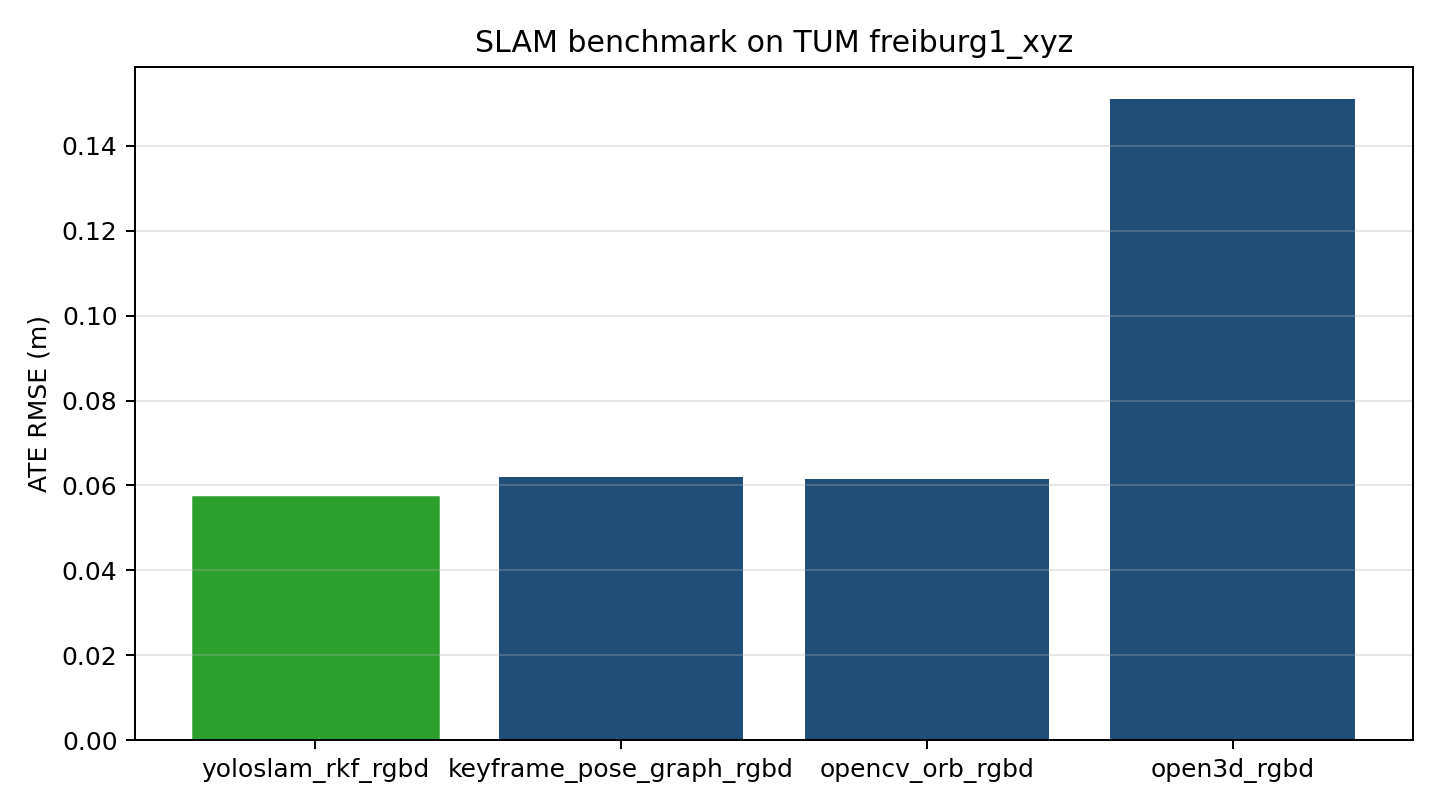
\includegraphics[width=0.92\linewidth]{figures/slam_ate_bar.png}
\caption{SLAM ATE RMSE on TUM RGB-D freiburg1\_xyz.}
\label{fig:slam_bar}
\end{figure}

\begin{figure}[t]
\centering
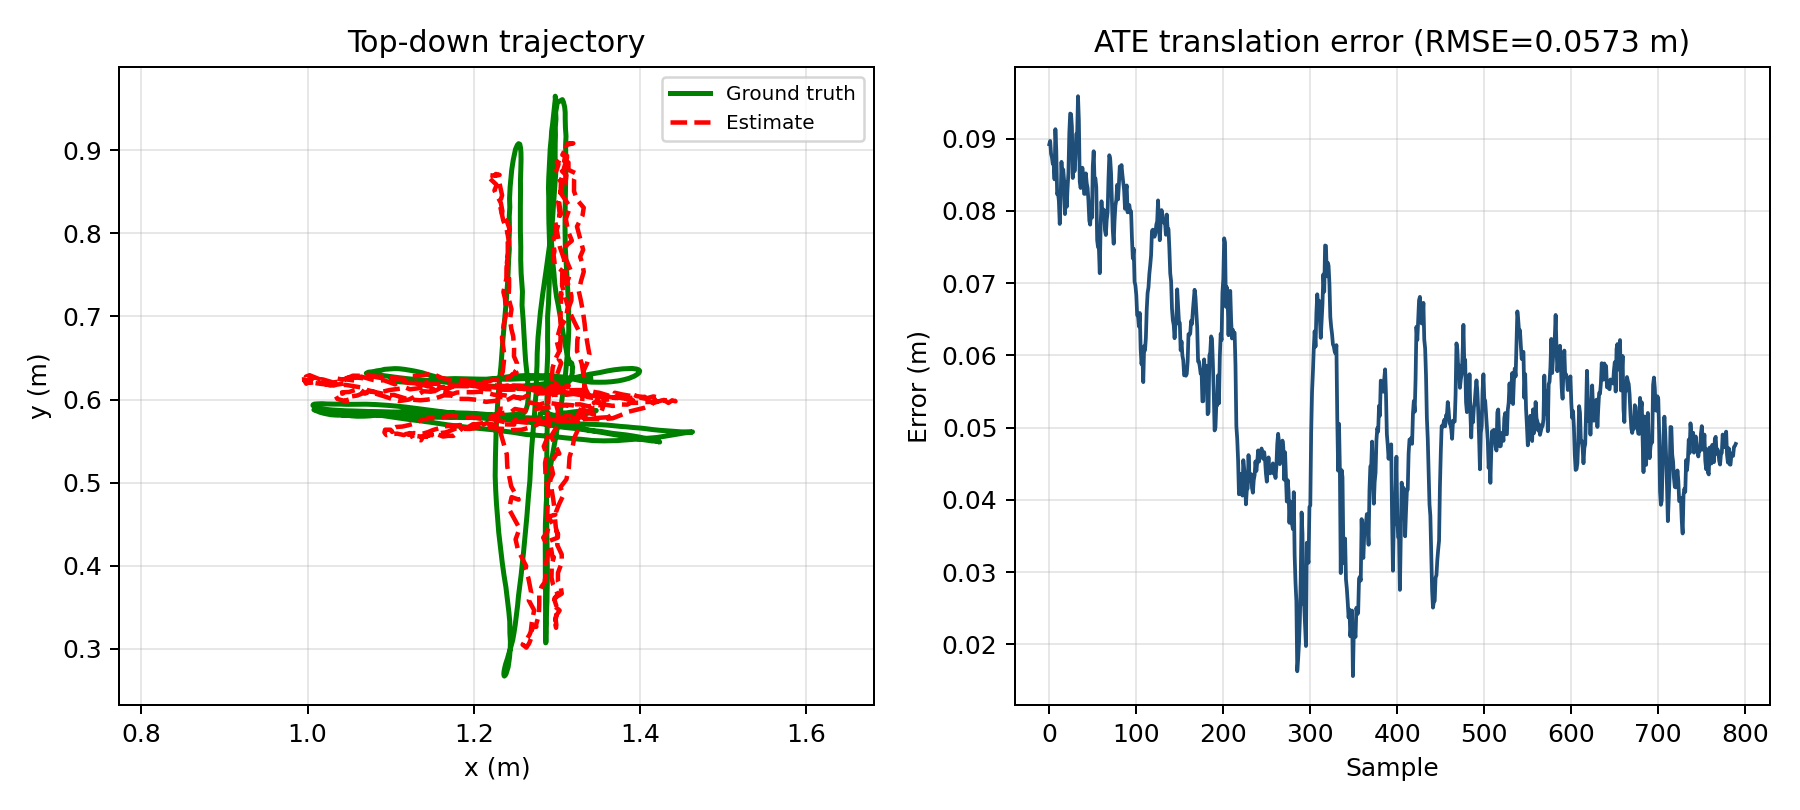
\includegraphics[width=0.92\linewidth]{figures/slam_trajectory.png}
\caption{Estimated vs.\ ground-truth trajectory (keyframe ORB RGB-D, evo).}
\label{fig:slam_traj}
\end{figure}

\subsection{Landing and safety controller}
Table~\ref{tab:landing} reports PyBullet batch metrics over five random seeds (normal landing, no injected abort). All trials selected a safe zone and completed touchdown. Abort trials (same seeds, hazard injected at descent) triggered ABORT on the same timestep as injection (0\,s latency).

\begin{table}[t]
\centering
\caption{PyBullet landing pipeline (5 seeds, semantic fusion + SLAM).}
\label{tab:landing}
\begin{tabular}{lc}
\toprule
Metric & Result \\
\midrule
Grid convergence time & $17.3 \pm 1.2$\,s \\
Time to land & $35.4 \pm 2.3$\,s \\
Zone accuracy at touchdown & 100\% \\
Abort detection latency & 0.0\,s \\
\bottomrule
\end{tabular}
\end{table}

Fig.~\ref{fig:pipeline} shows safety-map evolution, controller states, and representative nadir views. Fig.~\ref{fig:abort} shows climb after dynamic abort when a hazard enters the committed zone.

\begin{figure*}[t]
\centering
\begin{subfigure}[b]{0.24\textwidth}
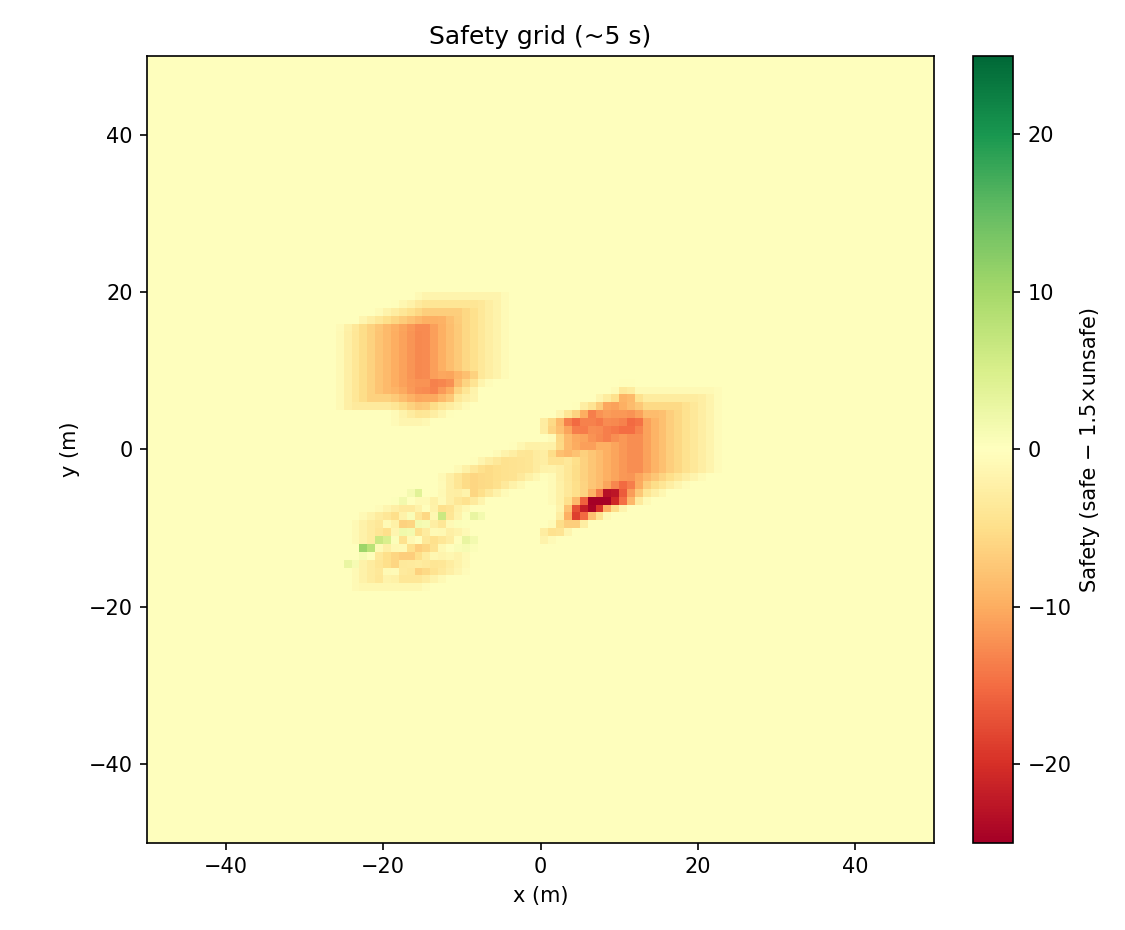
\includegraphics[width=\linewidth]{figures/grid_t05.png}
\caption{Survey ($t{=}5$\,s)}
\end{subfigure}
\hfill
\begin{subfigure}[b]{0.24\textwidth}
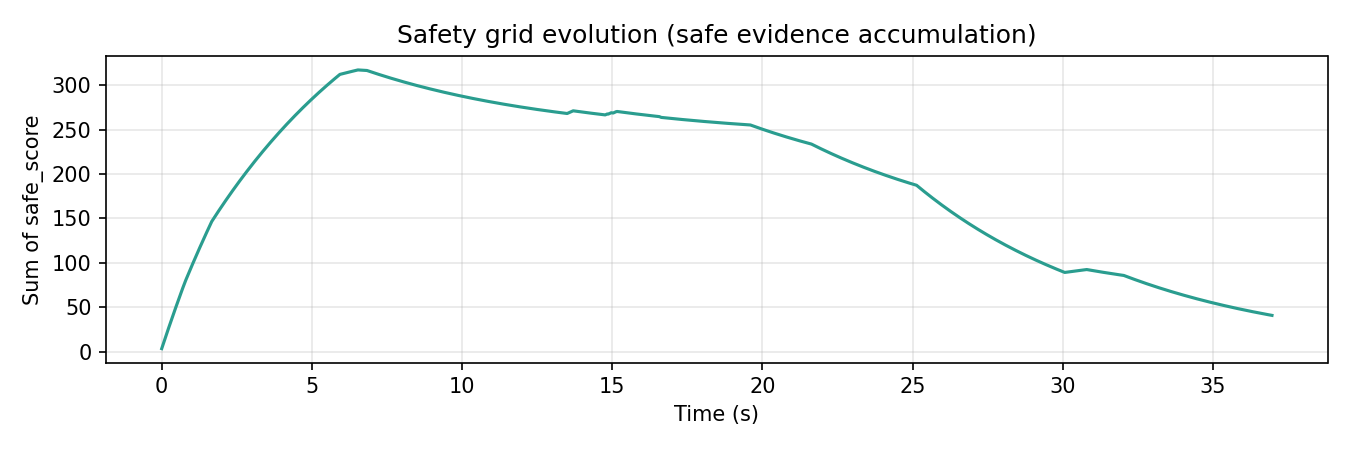
\includegraphics[width=\linewidth]{figures/grid_evolution.png}
\caption{Safety map evolution}
\end{subfigure}
\hfill
\begin{subfigure}[b]{0.24\textwidth}
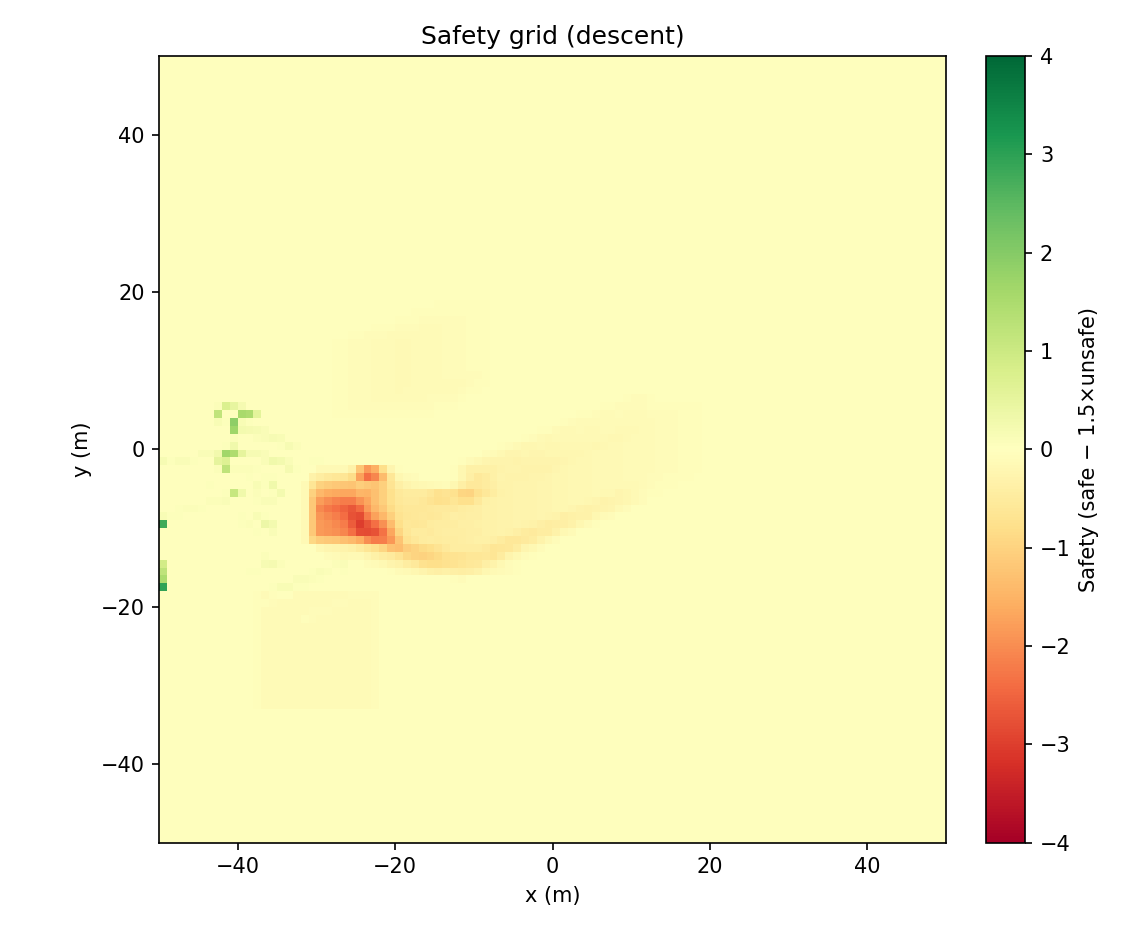
\includegraphics[width=\linewidth]{figures/grid_descent.png}
\caption{Descent phase}
\end{subfigure}
\hfill
\begin{subfigure}[b]{0.27\textwidth}
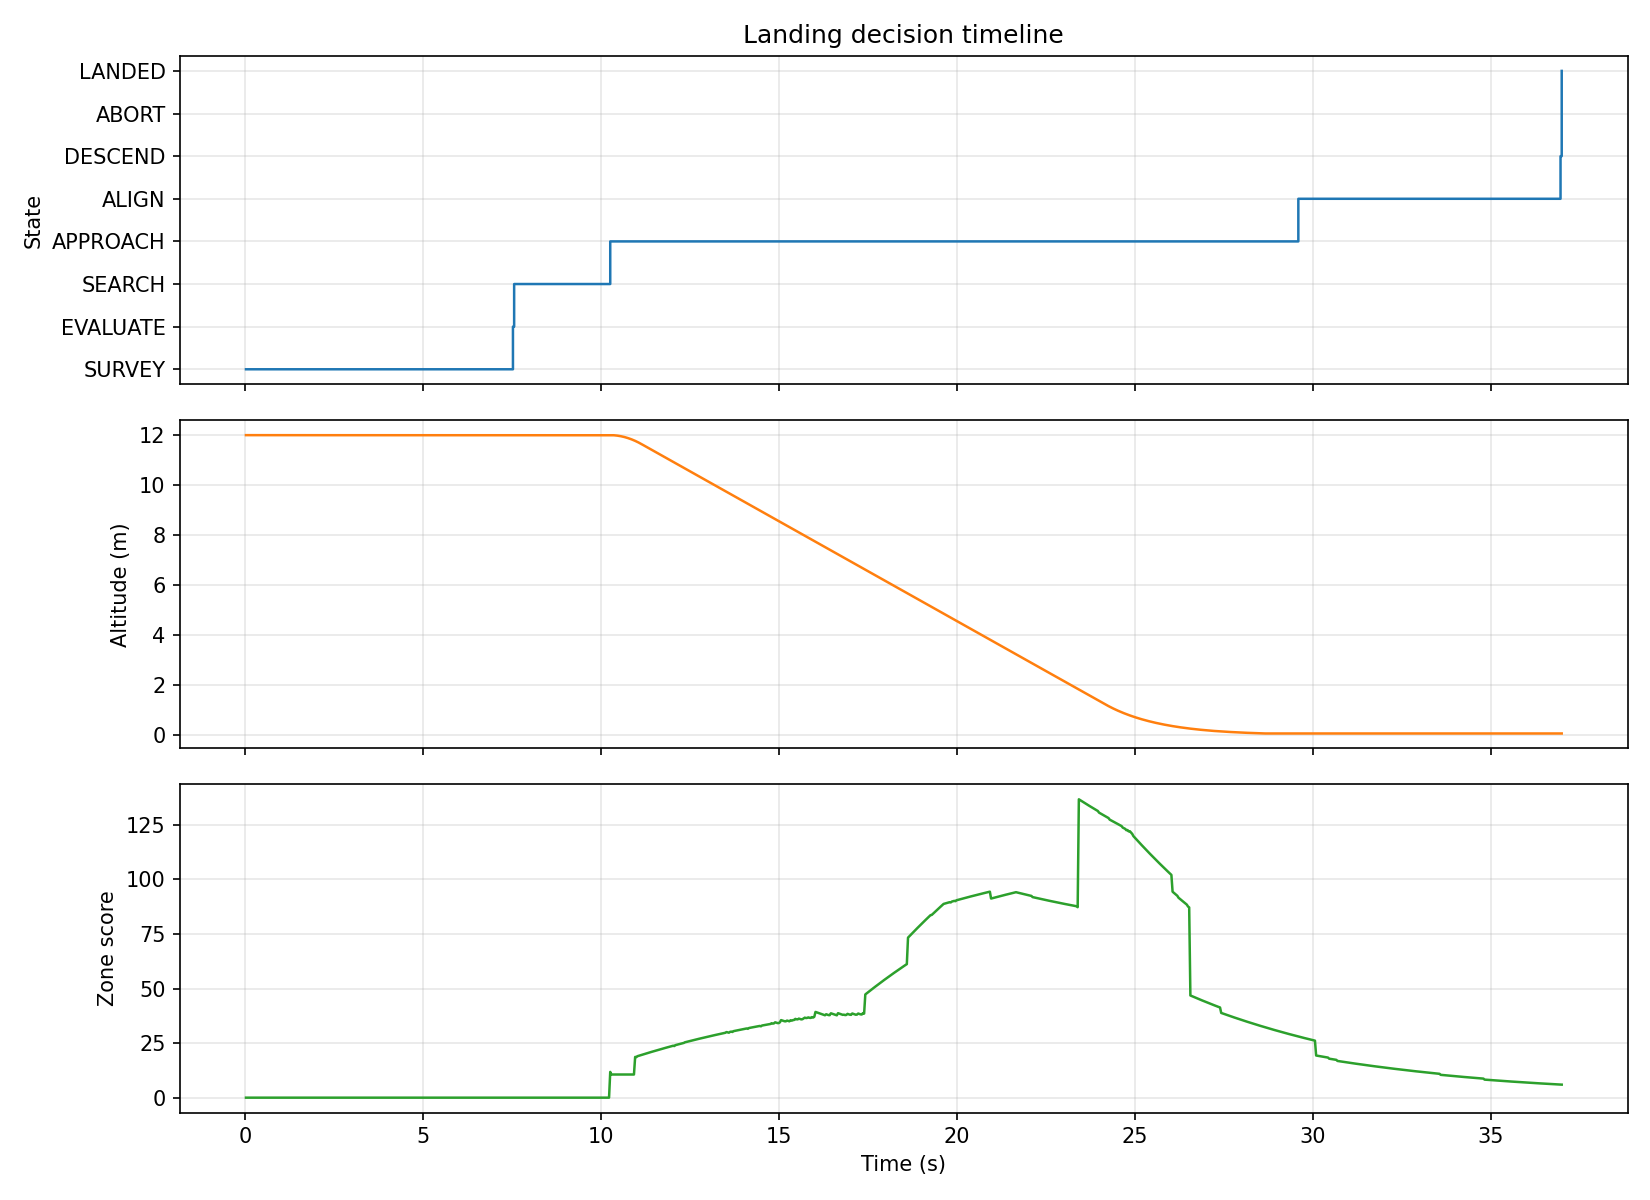
\includegraphics[width=\linewidth]{figures/decision_timeline.png}
\caption{Controller FSM}
\end{subfigure}
\caption{Semantic safety grid and controller timeline during a successful landing (seed 42).}
\label{fig:pipeline}
\end{figure*}

\begin{figure}[t]
\centering
\begin{subfigure}[b]{0.48\linewidth}
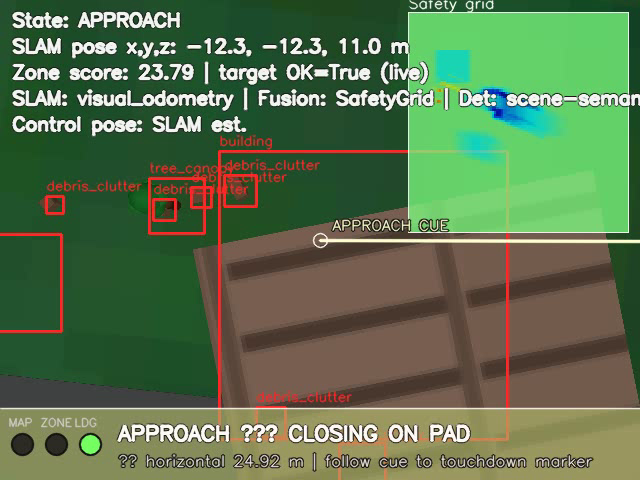
\includegraphics[width=\linewidth]{figures/pov_survey.png}
\caption{Nadir survey}
\end{subfigure}
\hfill
\begin{subfigure}[b]{0.48\linewidth}
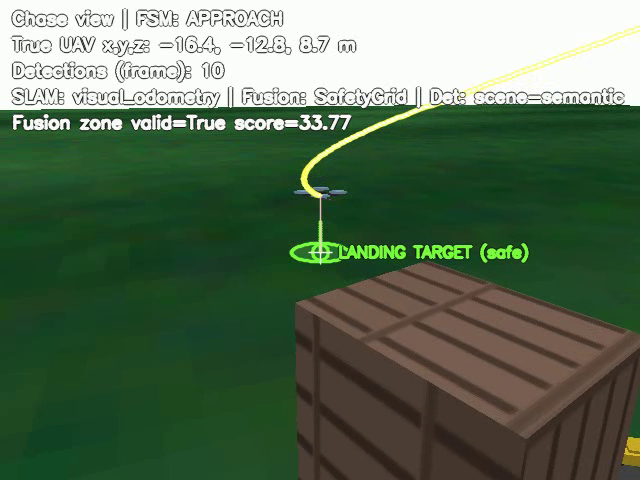
\includegraphics[width=\linewidth]{figures/abort_frame.png}
\caption{Abort + climb}
\end{subfigure}
\caption{Representative nadir view and abort response.}
\label{fig:abort}
\end{figure}

\section{Discussion}
Moving from marker-centric tracking to infrastructure-free landing requires both semantic reasoning and stable world-frame geometry. Benchmark-driven SLAM integration on commodity hardware, combined with persistent safety scoring, yields sub-10\,cm ATE on a standard RGB-D sequence and reliable simulated landings. External GPU SLAM systems remain future comparison targets on Linux hosts with CUDA.

\section{Conclusion}
Semantic-geometric fusion with persistent safety scoring and benchmark-selected RGB-D SLAM is a strong path toward robust UAV landing without scene instrumentation.

\bibliographystyle{IEEEtran}
\bibliography{references}
\end{document}
